% XCircuit output "asdas2.tex" for LaTeX input from asdas2.eps
\def\putbox#1#2#3#4{\makebox[0in][l]{\makebox[#1][l]{}\raisebox{\baselineskip}[0in][0in]{\raisebox{#2}[0in][0in]{\scalebox{#3}{#4}}}}}
\def\rightbox#1{\makebox[0in][r]{#1}}
\def\centbox#1{\makebox[0in]{#1}}
\def\topbox#1{\raisebox{-0.60\baselineskip}[0in][0in]{#1}}
\def\midbox#1{\raisebox{-0.20\baselineskip}[0in][0in]{#1}}
   \scalebox{1.248}{
   \normalsize
   \parbox{5.95313in}{
   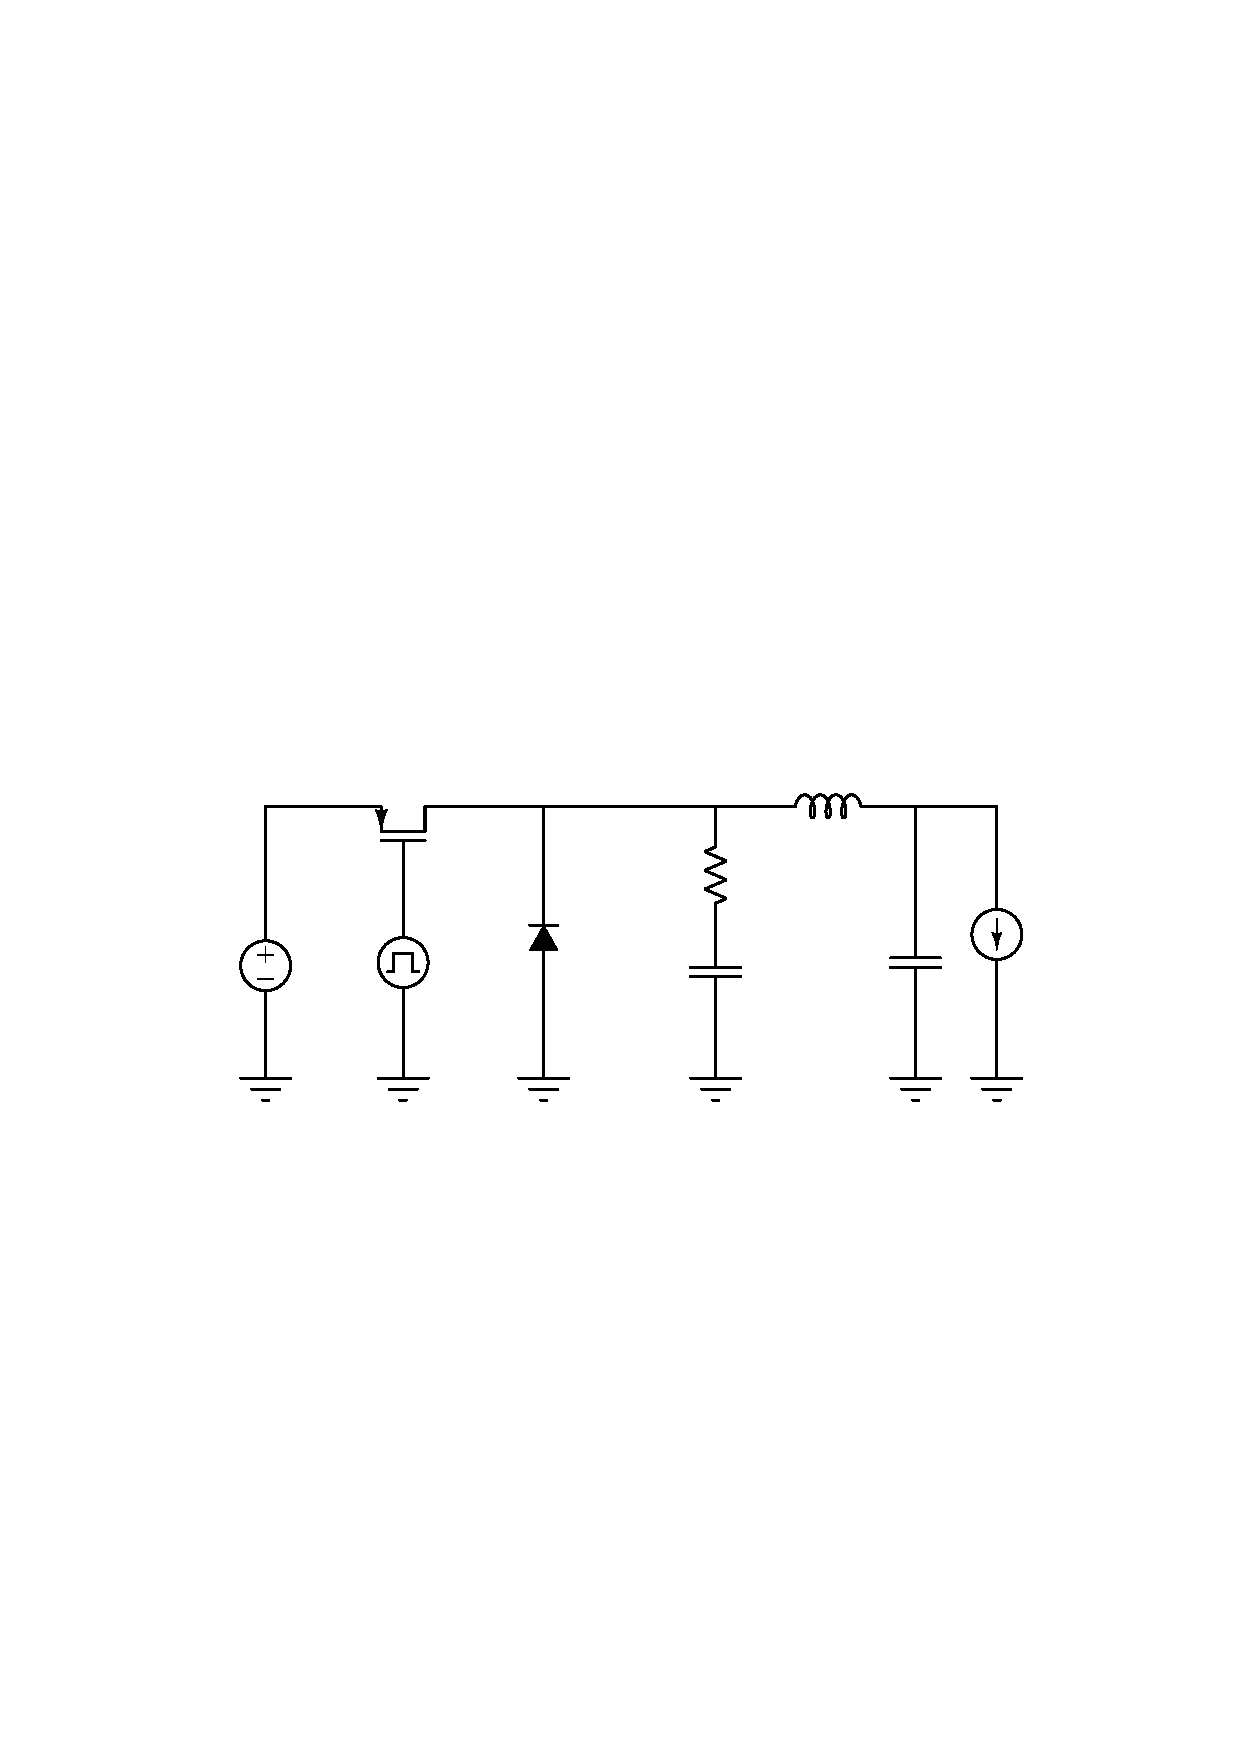
\includegraphics[scale=0.801282]{asdas}\\
   % translate x=901 y=341 scale 0.47
   \putbox{4.50in}{0.89in}{1.20}{C1}%
   \putbox{1.35in}{2.10in}{1.20}{M1}%
   \putbox{0.12in}{1.12in}{1.20}{V1}%
   \putbox{0.04in}{0.81in}{1.20}{12V}%
   \putbox{1.02in}{0.96in}{1.20}{V2}%
   \putbox{0.83in}{0.58in}{1.20}{20kHz}%
   \putbox{2.06in}{1.04in}{1.20}{D1}%
   \putbox{4.21in}{2.21in}{1.20}{L1}%
   \putbox{4.21in}{1.73in}{1.20}{10u}%
   \putbox{3.12in}{0.87in}{1.20}{C3}%
   \putbox{3.21in}{0.54in}{1.20}{5n}%
   \putbox{3.17in}{1.48in}{1.20}{R6}%
   \putbox{3.75in}{1.50in}{1.20}{100}%
   \putbox{5.73in}{1.06in}{1.20}{2A}%
   \putbox{4.56in}{0.67in}{1.20}{1m}%
   } % close 'parbox'
   } % close 'scalebox'
   \vspace{-\baselineskip} % this is not necessary, but looks better
